\documentclass[11pt,a4paper,titlepage]{article}

% Font related packages
\usepackage{fontspec}
\setmainfont{Lato}
\setsansfont{Lato}
\setmonofont{Fira Mono}
\newfontfamily\greekfont[Script=Greek]{Lato}

% Greek monospace font
\newfontfamily{\greekfonttt}{Fira Mono}
\usepackage{polyglossia}
\setdefaultlanguage{greek}

% Math packages
\usepackage{amsmath}
\usepackage{amsfonts}
\usepackage{amssymb}
\usepackage{makeidx}
\usepackage{eurosym}

% Graphics
\usepackage{graphicx}
\usepackage{float}
\usepackage{tikz}
\usetikzlibrary{arrows,positioning,shapes}

\usepackage{appendix} % Add appendix to document
\usepackage[margin=3cm]{geometry} % Change page margins

% Table packages
\usepackage{multirow}
\usepackage{color, colortbl}
\usepackage{array}
\usepackage{longtable}
\usepackage{lscape}

% PDF options
\usepackage[unicode,hidelinks,pdftitle={Ανάπτυξη συστήματος με υλοποίηση μεθοδολογίας MINORA (UTA) σε περιβάλλον Python με web interface},pdfauthor={Dimitrios Maroulidis, Myron Pachakis},pdfcreator={},pdfproducer={}]{hyperref}

% Colors to use in tables
\definecolor{LightGray}{gray}{0.95}
\definecolor{Gray}{gray}{0.9}
\definecolor{LightRed}{HTML}{ff6b6b}
%\definecolor{LightBlue}{HTML}{aacfff}
%\definecolor{LightBlue}{HTML}{5eaeff}
\definecolor{LightBlue}{HTML}{a7d2ff}

% Table column types for math environments
\newcolumntype{e}{>{$}c<{$}}
\renewcommand{\arraystretch}{1.2}
\usepackage{ragged2e}

% Math font
\usepackage{unicode-math}
\setmathfont{Asana Math}
% Use section based numbering for equations.
% amsmath is needed for this.
\numberwithin{equation}{section}

% Use comma as decimal point
%\usepackage{icomma}

% Code highlighting
\usepackage{minted}

% Comments
\usepackage{comment}

\author{Δημήτριος Μαρουλίδης (\textit{2018010111}) \and
    Μύρων Παχάκης (\textit{2018010028})}
\title{Ανάπτυξη συστήματος με υλοποίηση μεθοδολογίας MINORA (UTA) σε περιβάλλον Python με web interface}
\date{\today}

\begin{document}
\maketitle	
\tableofcontents
%	\listoffigures
%	\listoftables

\clearpage
% BEGIN HERE

\begin{comment}
Πλάνο Σύνταξης Αναφοράς
Εισαγωγή
1.Αντικειμενικοί Στόχοι Εργασίας-Προγράμματος
2.Περιγραφή μεθόδου θεωρητικά (Λογική της μεθόδου, ποιός την έφτιαξε)
3.Αναλύτικη Περιγραφή Μεθόδου (Χρησιμοποιούμε αυτό, κάνουμε αυτό, παρουσίαση αποτελέσματος, δεν σταματάμε όμως εκεί έχουμε ανατροφοδότηση από τον χρήστη (web interface), κάνει αυτή τη διαδικασία ο χρήστης)
4.Περιγραφή Υλοποίησης
5.Αναλυτικό Παράδειγμα εφαρμογής της μεθόδου
6.Παράρτημα -> Οδηγίες Χρήσης του προγράμματος-μεθόδου
7.Συμπεράσματα
8.Βιβλιογραφία
\end{comment}

\begin{abstract}
Η εργασία παρουσιάζει τη δημιουργία ενός αλληλεπιδραστικού προγράμματος στη γλώσσα προγραμματισμού Python για την επίλυση πολυκριτήριων συστήματων υποστήριξης αποφάσεων χρησιμοποιώντας το σύστημα MINORA. Για την υλοποίηση του συστήματος MINORA θα γίνει, επίσης, χρήση της μεθόδου πολυκριτήριας ανάλυσης UTASTAR. 

Η εργασία χωρίζεται σε δύο μέρη, το θεωρητικό αποτελείται από τα Κεφάλαια (1-3) και το προγραμματιστικό από τα Κεφάλαια (4-7). Στο Κεφάλαιο 1 παρουσιάζονται οι αντικειμενικοί στόχοι που αναμένονται από το πρόγραμμα. Στο Κεφάλαιο 2 περιγράφεται αναλυτικά η θεωρία πίσω από την μέθοδο UTASTAR και το σύστημα MINORA όπως η λογική λειτουργίας και ο τρόπος χρήσης τους, καθώς και οι πρωτοπόροι υλοποίησης και παρουσίασης των μεθόδων. Στο Κεφάλαιο 3 γίνεται αναλυτική παρουσίαση βήμα-βήμα στη εφαρμογή των μεθόδων UTA-UTASTAR-MINORA.

Στο Κεφάλαιο 4 αναλύεται διεξοδικά το πρόγραμμα σε γλώσσα Python καθώς και η αλληλεπίδραση μέσω του web interface, ενώ στο Κεφάλαιο 5 δίνεται ένα παράδειγμα πολυκριτήριων αποφάσεων και εφαρμόζεται η μέθοδος MINORA. Στο Κεφάλαιο 6 εντοπίζονται εκτενείς οδηγίες χρήσης του προγράμματος και στο Κεφάλαιο 7 συνοψίζονται τα συμπεράσματα της εργασίας και της χρήσης των μεθόδων-προγράμματος. Στο Κεφάλαιο 8 δίνεται η σχετική βιβλιογραφία και οι πηγές που χρησιμοποιήθηκαν.
\end{abstract}


%Μία πρώτη προσπάθεια είναι, δες ότι δεν σου αρέσει ή οτι θες να αλλάξουμε (πιθανών και να γραψουμε λιγα παραπανω?) Επίσης όπου υπάρχουν οι αριθμοί των κεφαλαίων θα αλλάξουν με τα tags των sectors για να μην γινεται μπερδεμα.  

\section{Αντικειμενικοί Στόχοι}
\label{sec:1}   
\begin{itemize}
	\item Συγγραφή ενός προγράμματος σε γλώσσα προγραμματισμού Python με σκοπό την υποστήριξη για τη λήψη αποφάσεων από τον χρήστη.
	\item Υλοποίηση συστήματος MINORA της οποίας το αποτέλεσμα είναι ένα μοντέλο το οποίο μοντελοποιεί τη διαδικασία απόφασης όσο πιο πιστά γίνεται.
	\item Παρουσίαση σε απλή και ευανάγνωστη μορφή του αποτελέσματος.
	\item Δυνατότητα άμεσης αλληλεπίδρασης του χρήστη με το πρόγραμμα μέσω web interface.
	\item Επίδειξη αναλυτικών οδηγιών χρήσης του προγράμματος.
\end{itemize}


\section{Θεωρητική Περιγραφή Μεθόδου}
\label{sec:2}
Η μέθοδος πολυκριτήριας ανάλυσης UTASTAR (UTilités Additives *) είναι υπεύθυνη για την εκτίμηση μίας ή παραπάνω συναρτήσεων αξίας χρησιμοποιώντας διαδικασίες γραμμικού προγραμματισμού. Στόχος των συναρτήσεων αξίας που θα εξαχθούν είναι η όσο το δυνατόν καλύτερη κατάταξη κάποιων επιλογών $a$ σε σύγκριση με την αρχική κατάταξη που έχει δωθεί από τον χρήστη. Ο χρήστης είναι υπεύθυνος για την εισαγωγή ενός συνόλου επιλογών $A_{R}$ κατανεμημένου με σειρά προτίμησης καθώς επίσης και ενός συνόλου κριτηρίων επιλογής $g_{n}$. 

Το σύστημα MINORA (Multicriteria Interactive Ordinal Regression Analysis), χρησιμοποιεί την μέθοδο UTASTAR για την εξαγωγή της λύσης του πολυκριτήριου προβλήματος, με την διαφορά ότι το σύστημα δίνει την δυνατότητα στον χρήστη να ανατροφοδοτήσει τυχόν δεδομένα, καταλήγοντας στο επιθυμητό σύστημα προτιμήσεων.

Πρωτοπόροι επιμελητές της μεθόδου UTASTAR είναι οι καθηγητές Siskos, Y. και Yannacopoulos, D., το 1985, ενώ το σύστημα MINORA επιμελήθηκε από τον καθηγητή Siskos, Y. και συνεργάτες, το 1993 και το 1994. 

%Δεν έχω αναφέρει πουθενά την UTA, θεωρείς ότι πρέπει να την αναφέρουμε?
\newpage

\section{Αναλυτική Περιγραφή Μεθόδου}
\label{sec:3}
Όπως έχει ήδη ειπωθεί ο χρήστης παρέχει ένα σύνολο $A_{R}$ εναλλακτικών επιλογών $a$ κατανεμημένων με σειρά προτίμησης από το καλύτερο στο χειρότερο καθώς επίσης και ένα σύνολο κριτηρίων $g_{n}$. Ανάλογα με τον αριθμό των επιλογών, θα χωριστούν ισαπέχοντα διαστήματα για κάθε κριτήριο χωριστά: 

\begin{equation}\label{initial_inter}
[g_{i*},g^{*}_{i}] = [g^{1}_{i}, ..., g^{a_{i}}_{i}]
\end{equation}
όπου $g^{a_{i}}_{i}$ οι διάφορες τιμές του συγκεκριμένου κριτηρίου, $g_{i*}$ η χειρότερη τιμή του συγκεκριμένου κριτηρίου και $g^{*}_{i}$ η καλύτερη τιμή του συγκεκριμένου κριτηρίου. 	
Σε αυτό το σημείο είναι απαραίτητο να γίνει ορισμός της έννοιας των χρησιμοτήτων των διαφόρων επιλογών $u(g(a))$, ο οποίος αποτελεί το μοντέλο απόφασης στην μέθοδο UTASTAR. Eκφράζεται ως μία προσθετική συνάρτηση των αύξουσων μερικών χρησιμοτήτων των κριτηρίων $u_{i}(g^{j}_{i})$:

\begin{equation}\label{total_uti}
	u(g(a)) = \sum_{i=1}^{n} u_{i}(g_{i}(a)) = u_{1}(g_{1}(a)) + u_{2}(g_{2}(a)) + ... + u_{n}(g_{n}(a))
\end{equation}
όπου $i = 1,2,...,n$ ο αριθμός του κριτηρίου και $a\in A_{R}$ η συγκεκριμένη επιλογή.

Λόγω του ότι ο χρήστης έχει κατατάξει τις επιλογές του κατά σειρά προτίμησης τότε είναι προφανές ότι η επιλογή $a_{m}$ θα είναι πάντα προτιμότερη ή ίση (αδιάφορη) από την επιλογή $a_{m+1}$.    

Είναι, λοιπόν, απαραίτητο να διατηρηθεί η μονοτονικότητα των κριτηρίων $g_{i}$. Έτσι με βάση την προτιμησιακή ανεξαρτησία των κριτηρίων η μονοτονία παραμένει ίδια τόσο στις μερικές συναρτήσεις χρησιμοτήτων $u_{i}(g^{j}_{i})$ όσο και στην ολική συνάρτηση  $u(g(a))$.

\centerline{Σε περίπτωση προτίμησης ισχύει: $u_{i}(g^{j+1}_{i}) > u_{i}(g^{j}_{i})$}

\centerline{Σε περίπτωση αδιαφορίας ισχύει: $u_{i}(g^{j+1}_{i}) = u_{i}(g^{j}_{i})$}

Στη συνεχεία ορίζονται οι μεταβλητές $w_{ij}$ σύμφωνα με τις παραπάνω σχέσεις μονοτονίας των κριτηρίων ως:

\begin{equation}\label{def_w}
	w_{ij} = u_{i}(g^{j+1}_{i}) - u_{i}(g^{j}_{i}) \geq 0
\end{equation}
όπου $i = 1,2,...,n$ και $j = 1,2,...,a_{i}-1$. Με αυτόν τον τρόπο είναι δυνατόν να αναπαρασταθεί η εξίσωση \ref{total_uti} των ολικών χρησιμοτήτων $u(g(a))$ με χρήση των μεταβλητών $w_{ij}$ αντί με χρήση των μερικών χρησιμοτήτων $u_{i}(g^{j}_{i})$. 

Για να πραγματοποιηθεί αυτή η μετατροπή είναι απαραίτητο να γίνει χρήση των παρακάτω σχέσεων:

\begin{equation}\label{zero_crit}
	u_{i}(g^{1}_{i}) = 0
\end{equation}

\begin{equation}\label{sum_w}
	u_{i}(g^{j}_{i}) = \sum_{i=1}^{j-1} w_{ij}
\end{equation}
όπου $i = 1,2,...,n$ και $j = 2,3,...,a_{i}-1$.

\newpage

Η εξίσωση \ref{zero_crit} είναι υπεύθυνη για τον μηδενισμό της χειρότερης τιμής του κάθε κριτηρίου ενώ στην εξίσωση \ref{sum_w} παρουσιάζεται η τιμή της χρησιμότητας του κάθε κριτηρίου ως το άθροισμα των μεταβλητών $w_{ij}$.  

Εάν οποιαδήποτε μερική χρησιμότητα $u_{i}(g_{i}(a))$ δεν υπάρχει στις διακριτές τιμές του αντίστοιχου κριτηρίου τότε είναι αναγκαίο να γίνει γραμμική παρεμβολή στο συγκεκριμένο κριτήριο $g_{i}^{j}$. 

Θεωρούνται πεπερασμένα τα άκρα $g_{i*}$ και $g^{*}_{i}$ του κριτηρίου και γίνεται χωρισμός του διαστήματος από την σχέση \ref{initial_inter} σε ισάριθμα υποδιαστήματα $(a_{i}-1)$, όπου το συγκεκριμένο σημείο που θα γίνει ο χωρισμός υπολογίζεται από τον τύπο:

\begin{equation}
	g_{i}^{j} = g_{i*} + \frac{j-1}{a_{i}-1}(g^{*}_{i}-g_{i*})
\end{equation}
για $j = 1,2,...,a_{i}$ και $g_{i*}$ η χειρότερη τιμή του συγκεκριμένου κριτηρίου και $g^{*}_{i}$ η καλύτερη τιμή του συγκεκριμένου κριτηρίου.

Η γραμμική παρεμβολή εφαρμόζεται σύμφωνα με τον τύπο \ref{linear_inter} και δίνει ως αποτέλεσμα την τιμή της μερικής χρησιμότητας για την επιλογή $a$.

\begin{equation}\label{linear_inter}
	u_{i}(g_{i}(a)) = u_{i}(g^{j}_{i}) + \frac{g_{i}(a)-g^{j}_{i}}{g^{j+1}-g^{j}_{i}}(u_{i}(g_{i}^{j+1})-u_{i}(g_{i}^{j}))
\end{equation}


Στη μέθοδο UTASTAR είναι απαραίτητο να χρησιμοποιηθεί μία διπλή συνάρτηση σφάλματος όπου θα εκφράζει το ποσό της χρησιμότητας που θα πρέπει να προστεθεί ή να αφαιρεθεί, αντίστοιχα, από την ολική χρησιμότητα $u(g(a))$ με σκοπό να είναι δυνατόν η επιλογή $a$ που έχει ως ολική χρησιμότητα την $u(g(a))$ να ανακατακτήσει την θέση της στη διάταξη των επιλογών.

Τα 2 σφάλματα αυτά ονομάζονται σφάλμα υποεκτίμησης $σ^{+}$ το οποίο αφαιρεί ένα ποσό αξίας και σφάλμα υπερεκτίμησης $σ^{-}$ το οποίο προσθέτει ένα ποσό αξίας.

Με αυτόν τον τρόπο τα σημεία των επιλογών $a$ σταθεροποιούνται με μεγαλύτερη ακρίβεια πάνω στην καμπύλη μονότονης παλινδρόμησης όπως παρουσιάζεται στο σχήμα \ref{fig:graph_monot}.

\begin{figure}[H]
	\centering
	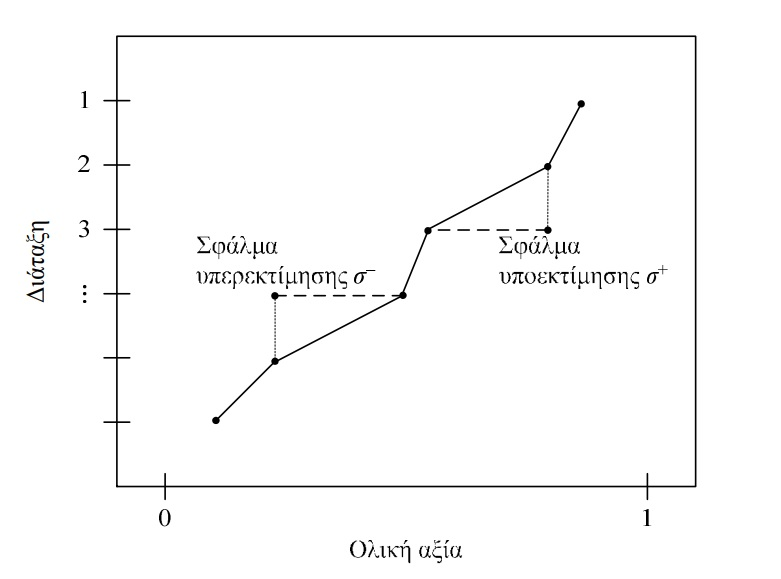
\includegraphics[width=0.7\linewidth]{media/graph_mono.jpg}
	\caption{Καμπύλη Μονότονης Παλινδρόμησης}
	\label{fig:graph_monot}
\end{figure}

Με τις παραπάνω προσθήκες των σφαλμάτων η εξίσωση των ολικών χρησιμοτήτων \ref{total_uti} μετατρέπεται σε:

\begin{equation}\label{total_uti_fin}
	u(g(a)) = \sum_{i=1}^{n} u_{i}(g_{i}(a)) - σ^{+}(a) + σ^{-}(a)
\end{equation}
όπου $i = 1,2,...,n$ ο αριθμός του κριτηρίου και $a\in A_{R}$ η συγκεκριμένη επιλογή.

Έτσι για δύο διαδοχικές επιλογές $a_{m}$ και $a_{m+1}$ ορίζεται:

\begin{equation}\label{def_deltas}
	Δ(a_{m}, a_{m+1}) = u(g(a_{m})) - σ^{+}(a_{m}) + σ^{-}(a_{m}) - u(g(a_{m+1})) + σ^{+}(a_{m+1}) - σ^{-}(a_{m+1})
\end{equation}

Όπου οι χρησιμότητες $u(g(a_{m}))$ μπορούν να αντικατασταθούν από τις μεταβλητές $w_{ij}$ με βάση τις σχέσεις \ref{def_w} και \ref{sum_w}.
 
Έχει ήδη αναφερθεί πως η μέθοδος UTASTAR χρησιμοποιεί μεθόδους γραμμικού προγραμματισμού για τον υπολογισμό των μερικών συναρτήσεων χρησιμότητας-αξίας. Επιλύεται το παρακάτω γραμμικό πρόβλημα με αντικειμενική συνάρτηση ελαχιστοποίησης των συνολικών σφαλμάτων $σ^{+}$ και $σ^{-}$.

\begin{equation}\label{linear_program}
	\begin{aligned}
	&[min] F = \sum_{a\in A_{R}} {σ^{+}(a) + σ^{-}(a)} \\
	&\text{υπό περιορισμούς}\\
	&Δ(a_{m},a_{m+1}) \geq δ ~\text{εάν}~ a_{m}\succ a_{m+1}\\
	&Δ(a_{m},a_{m+1}) = 0 ~\text{εάν}~ a_{m}\sim a_{m+1}\\
	&\sum_{n}^{i=1}\sum_{j=1}^{a_{i}-1} w_{ij} = 1\\
	& w_{ij} \geq 0, σ^{+}(a) \geq 0, σ^{-}(a) \geq 0 \forall a\in A_{R}, \forall i,j
	\end{aligned}
\end{equation}
 
\newpage

Όπου $δ$ ορίζεται ως η τιμή του κατωφλιού προτίμησης και έχει μία μικρή θετική τιμή. Εξασφαλίζει ότι η διάταξη των εναλλακτικών ταιριάζει με το μοντέλο προτιμήσεων του αποφασίζοντα.

Αφού εξαχθεί η λύση του γραμμικού προγράμματος τότε γίνεται ανάλυση ευστάθειας, δηλαδή ελέγχουμε εάν υπάρχουν περισσότερες από μία βέλτιστες λύσεις ή εάν υπάρχουν λύσεις που είναι πολύ κοντά στη βέλτιστη που έχουμε υπολογίσει.

Σε περίπτωση όπου η βέλτιστη λύση της αντικειμενικής συνάρτησης έχει τιμή μηδέν τότε υπάρχουν παραπάνω από μία λύσεις που ικανοποιούν την διάταξη επιλογών $A_{R}$ που έχει εισάγει ο χρήστης. Επίσης υπολογίζουμε τη μέση τιμή των συναρτήσεων χρησιμότητας εκείνων των κοντινότερων βέλτιστων λύσεων που μεγιστοποιούν τις αντικειμενικές συναρτήσεις:

\begin{equation}
	u_{i}(g_{i}^{*}) = \sum_{j=1}^{a_{i}-1} w_{ij}  ~~\forall i=1,2,..,n
\end{equation} 

Η αντικειμενική συνάρτηση του αρχικού γραμμικού προγράμματος \ref{linear_program} θέτεται ως περιορισμός:

\begin{equation}
	\sum_{a\in A_{R}} {σ^{+}(a) + σ^{-}(a)} \leq z^{*} + ε
\end{equation}

Όπου $z_{*}$ είναι η βέλτιστη τιμή του αρχικού γραμμικού \ref{linear_program}, δηλαδή το ελάχιστο σφάλμα, και $ε$ είναι είτε μηδέν είτε ένας μικρός θετικός αριθμός. 

Όταν υπάρχει αστάθεια οι βέλτιστες λύσεις των γραμμικών προγραμμάτων παρουσιάζουν μεγάλη απόκλιση μεταξύ τους, γεγονός το οποίο οδηγεί σε μεγαλύτερη διακύμανση των μεταβλητών $w_{ij}$. Με αυτόν τον τρόπο μπορούμε να καταλάβουμε πόσο σημαντικό είναι το κάθε κριτήριο $g_{i}$ στη διάταξη επιλογών που έχει ορίσει ο χρήστης.



\end{document}